\section{Learning Objectives}

After completing this chapter, readers will be able to:
\begin{itemize}
    \item Design data pipeline architectures for batch, streaming, and real-time ML workloads
    \item Choose between ETL and ELT patterns based on ML requirements
    \item Implement comprehensive data validation using Great Expectations
    \item Build and operate feature stores for ML feature management
    \item Handle schema evolution and ensure backward compatibility
    \item Use Apache Beam for portable data processing pipelines
    \item Integrate Kafka for streaming data ingestion
    \item Version datasets and track data lineage with DVC
    \item Monitor data quality and detect data drift
    \item Design fault-tolerant, scalable data pipelines
\end{itemize}

\section{Introduction: Data Pipelines as the Foundation}

Data pipelines form the critical foundation of any production ML system. While models receive the majority of attention, the reality is that 80\% of ML engineering effort goes into data preparation, quality assurance, and pipeline maintenance \citep{cognilytica2020}.

A robust data pipeline must address several challenges simultaneously:

\begin{itemize}
    \item \textbf{Scale:} Processing gigabytes to petabytes of data efficiently
    \item \textbf{Reliability:} Ensuring consistent, accurate data delivery
    \item \textbf{Latency:} Meeting timing requirements from batch to real-time
    \item \textbf{Quality:} Validating data and detecting anomalies
    \item \textbf{Versioning:} Tracking data evolution and enabling reproducibility
    \item \textbf{Governance:} Ensuring privacy, security, and compliance
\end{itemize}

\section{Data Ingestion Patterns}

Data ingestion represents the entry point for raw data into the ML system. The choice of ingestion pattern fundamentally shapes the architecture, latency characteristics, and operational complexity of the entire pipeline.

\subsection{Batch Processing}

Batch processing handles data in discrete chunks on a scheduled basis. This pattern suits scenarios where:
\begin{itemize}
    \item Data naturally accumulates over time (daily logs, transactions)
    \item Processing large volumes efficiently is more important than latency
    \item Complex transformations require access to full datasets
    \item Cost optimization favors periodic processing over continuous operations
\end{itemize}

\begin{figure}[h]
\centering
\begin{tikzpicture}[node distance=2.5cm, auto]
    \tikzstyle{source} = [rectangle, rounded corners, draw, fill=blue!20, text width=2.5cm, text centered, minimum height=1cm]
    \tikzstyle{process} = [rectangle, draw, fill=green!20, text width=2.5cm, text centered, minimum height=1cm]
    \tikzstyle{store} = [cylinder, draw, fill=orange!20, text width=2cm, text centered, minimum height=1.2cm, shape aspect=0.3]
    \tikzstyle{arrow} = [thick,->,>=stealth]

    \node [source] (source) {Data Sources\\(DB, Logs, APIs)};
    \node [process, right of=source, node distance=3.5cm] (extract) {Extract\\(Scheduled)};
    \node [process, right of=extract, node distance=3.5cm] (transform) {Transform\\(Batch Job)};
    \node [process, right of=transform, node distance=3.5cm] (validate) {Validate\\(Quality Checks)};
    \node [store, right of=validate, node distance=3.5cm] (warehouse) {Data\\Warehouse};

    \draw [arrow] (source) -- (extract);
    \draw [arrow] (extract) -- (transform);
    \draw [arrow] (transform) -- (validate);
    \draw [arrow] (validate) -- (warehouse);

    \node [below of=extract, node distance=1.5cm] {Schedule: Daily/Hourly};
    \node [below of=transform, node distance=1.5cm] {Distributed Processing};
\end{tikzpicture}
\caption{Batch processing pipeline architecture}
\label{fig:batch_pipeline}
\end{figure}

\textbf{Apache Beam Batch Pipeline:}

\begin{lstlisting}[style=python, caption=Apache Beam batch processing pipeline]
import apache_beam as beam
from apache_beam.options.pipeline_options import PipelineOptions
from apache_beam.io import ReadFromText, WriteToBigQuery
import json

class ParseLogLine(beam.DoFn):
    """Parse raw log lines into structured records"""
    def process(self, element):
        try:
            record = json.loads(element)
            yield {
                'user_id': record['user_id'],
                'timestamp': record['timestamp'],
                'event_type': record['event_type'],
                'page_url': record.get('page_url', ''),
                'duration_ms': int(record.get('duration_ms', 0))
            }
        except (json.JSONDecodeError, KeyError) as e:
            # Log errors to side output
            yield beam.pvalue.TaggedOutput('errors', element)

class ExtractFeatures(beam.DoFn):
    """Extract ML features from parsed records"""
    def process(self, element):
        features = {
            'user_id': element['user_id'],
            'date': element['timestamp'][:10],
            'total_events': 1,
            'avg_duration_ms': element['duration_ms'],
            'unique_pages': 1 if element['page_url'] else 0
        }
        yield (element['user_id'] + '_' + features['date'], features)

class AggregateFeatures(beam.CombineFn):
    """Combine features per user per day"""
    def create_accumulator(self):
        return {
            'total_events': 0,
            'total_duration': 0,
            'pages': set()
        }

    def add_input(self, accumulator, element):
        accumulator['total_events'] += element['total_events']
        accumulator['total_duration'] += element['avg_duration_ms']
        if element['unique_pages']:
            accumulator['pages'].add(element.get('page_url', ''))
        return accumulator

    def merge_accumulators(self, accumulators):
        merged = self.create_accumulator()
        for acc in accumulators:
            merged['total_events'] += acc['total_events']
            merged['total_duration'] += acc['total_duration']
            merged['pages'].update(acc['pages'])
        return merged

    def extract_output(self, accumulator):
        return {
            'total_events': accumulator['total_events'],
            'avg_duration_ms': (accumulator['total_duration'] /
                              accumulator['total_events']
                              if accumulator['total_events'] > 0 else 0),
            'unique_pages': len(accumulator['pages'])
        }

def run_pipeline(input_path, output_table):
    """Execute the batch processing pipeline"""
    options = PipelineOptions([
        '--runner=DataflowRunner',
        '--project=my-gcp-project',
        '--region=us-central1',
        '--temp_location=gs://my-bucket/temp',
        '--max_num_workers=10',
        '--autoscaling_algorithm=THROUGHPUT_BASED'
    ])

    with beam.Pipeline(options=options) as pipeline:
        # Main processing branch
        parsed_data = (
            pipeline
            | 'ReadLogs' >> ReadFromText(input_path)
            | 'ParseLogs' >> beam.ParDo(ParseLogLine())
                .with_outputs('errors', main='parsed')
        )

        # Process valid records
        features = (
            parsed_data.parsed
            | 'ExtractFeatures' >> beam.ParDo(ExtractFeatures())
            | 'GroupByUserDate' >> beam.GroupByKey()
            | 'AggregateFeatures' >> beam.CombinePerKey(AggregateFeatures())
            | 'FormatOutput' >> beam.Map(
                lambda kv: {'user_date': kv[0], **kv[1]}
            )
            | 'WriteToBigQuery' >> WriteToBigQuery(
                output_table,
                schema='user_date:STRING,total_events:INTEGER,'
                       'avg_duration_ms:FLOAT,unique_pages:INTEGER',
                create_disposition=beam.io.BigQueryDisposition.CREATE_IF_NEEDED,
                write_disposition=beam.io.BigQueryDisposition.WRITE_APPEND
            )
        )

        # Log parsing errors
        errors = (
            parsed_data.errors
            | 'WriteErrors' >> beam.io.WriteToText(
                'gs://my-bucket/errors/batch-',
                file_name_suffix='.txt'
            )
        )

if __name__ == '__main__':
    run_pipeline(
        input_path='gs://my-bucket/logs/*.json',
        output_table='my-project:ml_features.user_daily_features'
    )
\end{lstlisting}

\subsection{Streaming Processing}

Streaming pipelines process data continuously as it arrives, enabling low-latency applications like fraud detection, recommendation systems, and real-time monitoring.

\begin{figure}[h]
\centering
\begin{tikzpicture}[node distance=2.5cm, auto]
    \tikzstyle{source} = [rectangle, rounded corners, draw, fill=blue!20, text width=2cm, text centered, minimum height=1cm]
    \tikzstyle{stream} = [rectangle, draw, fill=purple!20, text width=2cm, text centered, minimum height=1cm]
    \tikzstyle{process} = [rectangle, draw, fill=green!20, text width=2cm, text centered, minimum height=1cm]
    \tikzstyle{store} = [cylinder, draw, fill=orange!20, text width=1.8cm, text centered, minimum height=1cm, shape aspect=0.3]
    \tikzstyle{arrow} = [thick,->,>=stealth]

    \node [source] (app) {Applications};
    \node [stream, right of=app, node distance=3cm] (kafka) {Kafka\\Topics};
    \node [process, right of=kafka, node distance=3cm] (process) {Stream\\Processor};
    \node [store, below of=process, node distance=2cm] (feature) {Feature\\Store};
    \node [store, right of=process, node distance=3cm] (lake) {Data\\Lake};

    \draw [arrow] (app) -- (kafka) node[midway, above] {Events};
    \draw [arrow] (kafka) -- (process);
    \draw [arrow] (process) -- (feature);
    \draw [arrow] (process) -- (lake);

    \node [below of=kafka, node distance=1.5cm] {Real-time Buffer};
\end{tikzpicture}
\caption{Streaming pipeline architecture with Kafka}
\label{fig:streaming_pipeline}
\end{figure}

\textbf{Kafka Producer for Event Streaming:}

\begin{lstlisting}[style=python, caption=Kafka producer for streaming data ingestion]
from kafka import KafkaProducer
from kafka.errors import KafkaError
import json
import logging
from datetime import datetime
from typing import Dict, Any

logger = logging.getLogger(__name__)

class EventProducer:
    """Kafka producer for streaming ML events"""

    def __init__(self, bootstrap_servers: list, topic: str):
        self.topic = topic
        self.producer = KafkaProducer(
            bootstrap_servers=bootstrap_servers,
            value_serializer=lambda v: json.dumps(v).encode('utf-8'),
            key_serializer=lambda k: k.encode('utf-8') if k else None,
            # Performance tuning
            compression_type='snappy',
            batch_size=16384,
            linger_ms=10,
            # Reliability settings
            acks='all',
            retries=3,
            max_in_flight_requests_per_connection=5,
            # Idempotence for exactly-once semantics
            enable_idempotence=True
        )

    def send_event(self, user_id: str, event_data: Dict[str, Any]):
        """Send event to Kafka with error handling"""
        try:
            # Add metadata
            event = {
                'user_id': user_id,
                'timestamp': datetime.utcnow().isoformat(),
                **event_data
            }

            # Send with callback
            future = self.producer.send(
                self.topic,
                key=user_id,
                value=event,
                partition=None  # Let Kafka partition by key
            )

            # Optionally wait for confirmation
            record_metadata = future.get(timeout=10)
            logger.info(
                f"Event sent: topic={record_metadata.topic}, "
                f"partition={record_metadata.partition}, "
                f"offset={record_metadata.offset}"
            )

        except KafkaError as e:
            logger.error(f"Failed to send event: {e}")
            raise

    def close(self):
        """Flush and close producer"""
        self.producer.flush()
        self.producer.close()

# Usage example
if __name__ == '__main__':
    producer = EventProducer(
        bootstrap_servers=['localhost:9092'],
        topic='user_events'
    )

    try:
        # Simulate user events
        producer.send_event(
            user_id='user_12345',
            event_data={
                'event_type': 'page_view',
                'page_url': '/products/laptop',
                'duration_ms': 4532,
                'referrer': '/home'
            }
        )
    finally:
        producer.close()
\end{lstlisting}

\textbf{Kafka Consumer with Real-Time Feature Engineering:}

\begin{lstlisting}[style=python, caption=Kafka consumer for streaming feature processing]
from kafka import KafkaConsumer
from kafka.structs import TopicPartition
import json
import redis
from datetime import datetime, timedelta
from collections import defaultdict
import logging

logger = logging.getLogger(__name__)

class StreamingFeatureProcessor:
    """Process streaming events and compute real-time features"""

    def __init__(self, bootstrap_servers: list, topic: str,
                 redis_host: str = 'localhost'):
        # Kafka consumer
        self.consumer = KafkaConsumer(
            topic,
            bootstrap_servers=bootstrap_servers,
            group_id='feature_processor_group',
            value_deserializer=lambda m: json.loads(m.decode('utf-8')),
            key_deserializer=lambda k: k.decode('utf-8') if k else None,
            # Start from beginning if no offset
            auto_offset_reset='earliest',
            # Commit offsets automatically
            enable_auto_commit=True,
            auto_commit_interval_ms=5000,
            # Performance
            max_poll_records=500,
            session_timeout_ms=10000
        )

        # Redis for feature state
        self.redis = redis.Redis(
            host=redis_host,
            port=6379,
            decode_responses=True
        )

        # Local window state
        self.windows = defaultdict(list)
        self.window_size = timedelta(minutes=5)

    def compute_features(self, user_id: str, event: dict) -> dict:
        """Compute real-time features from event stream"""
        current_time = datetime.fromisoformat(event['timestamp'])

        # Get user's recent events from Redis
        recent_key = f"user:{user_id}:events:5min"
        recent_events = self.redis.lrange(recent_key, 0, -1)
        recent_events = [json.loads(e) for e in recent_events]

        # Add current event
        recent_events.append(event)

        # Compute features
        features = {
            'user_id': user_id,
            'timestamp': event['timestamp'],
            # Count features
            'events_5min': len(recent_events),
            'unique_pages_5min': len(set(
                e.get('page_url', '') for e in recent_events
            )),
            # Temporal features
            'avg_duration_5min': sum(
                e.get('duration_ms', 0) for e in recent_events
            ) / len(recent_events) if recent_events else 0,
            # Behavioral features
            'event_types_5min': list(set(
                e.get('event_type', '') for e in recent_events
            )),
            'is_high_activity': len(recent_events) > 10,
        }

        # Update Redis with sliding window
        self.redis.lpush(recent_key, json.dumps(event))
        self.redis.ltrim(recent_key, 0, 999)  # Keep last 1000
        self.redis.expire(recent_key, 300)  # 5 min TTL

        # Store computed features
        feature_key = f"user:{user_id}:features:latest"
        self.redis.setex(
            feature_key,
            300,  # 5 min TTL
            json.dumps(features)
        )

        return features

    def process_stream(self):
        """Main processing loop"""
        logger.info("Starting stream processor...")

        try:
            for message in self.consumer:
                try:
                    user_id = message.key
                    event = message.value

                    # Compute features
                    features = self.compute_features(user_id, event)

                    # Could publish to another topic, write to DB, etc.
                    logger.info(f"Processed features for {user_id}: "
                              f"{features['events_5min']} events in 5min")

                except Exception as e:
                    logger.error(f"Error processing message: {e}")
                    # Continue processing other messages

        except KeyboardInterrupt:
            logger.info("Shutting down processor...")
        finally:
            self.consumer.close()
            self.redis.close()

if __name__ == '__main__':
    processor = StreamingFeatureProcessor(
        bootstrap_servers=['localhost:9092'],
        topic='user_events',
        redis_host='localhost'
    )
    processor.process_stream()
\end{lstlisting}

\subsection{Micro-Batch Processing}

Micro-batching bridges batch and streaming by processing small batches at short intervals (seconds to minutes). This pattern, popularized by Apache Spark Streaming, provides a middle ground for many ML applications.

\begin{lstlisting}[style=python, caption=Apache Beam streaming pipeline with windowing]
import apache_beam as beam
from apache_beam.options.pipeline_options import PipelineOptions
from apache_beam.transforms.window import FixedWindows, TimestampedValue
from apache_beam.io import ReadFromPubSub, WriteToBigQuery
import json
from datetime import datetime

class ParseEvent(beam.DoFn):
    """Parse and enrich streaming events"""
    def process(self, element, timestamp=beam.DoFn.TimestampParam):
        try:
            event = json.loads(element.decode('utf-8'))
            yield TimestampedValue(event, timestamp.micros / 1000000)
        except json.JSONDecodeError:
            pass  # Skip malformed events

class ComputeWindowFeatures(beam.DoFn):
    """Compute features within time windows"""
    def process(self, element, window=beam.DoFn.WindowParam):
        user_id, events = element

        features = {
            'user_id': user_id,
            'window_start': window.start.to_utc_datetime().isoformat(),
            'window_end': window.end.to_utc_datetime().isoformat(),
            'event_count': len(events),
            'avg_duration': sum(e.get('duration_ms', 0)
                              for e in events) / len(events),
            'unique_pages': len(set(e.get('page_url', '')
                                  for e in events))
        }
        yield features

def run_streaming_pipeline(subscription: str, output_table: str):
    """Run streaming pipeline with windowing"""
    options = PipelineOptions([
        '--runner=DataflowRunner',
        '--project=my-gcp-project',
        '--region=us-central1',
        '--streaming',
        '--enable_streaming_engine'
    ])

    with beam.Pipeline(options=options) as pipeline:
        events = (
            pipeline
            | 'ReadFromPubSub' >> ReadFromPubSub(
                subscription=subscription
            )
            | 'ParseEvents' >> beam.ParDo(ParseEvent())
            | 'WindowInto' >> beam.WindowInto(
                FixedWindows(60)  # 1-minute windows
            )
            | 'KeyByUser' >> beam.Map(
                lambda e: (e['user_id'], e)
            )
            | 'GroupByUser' >> beam.GroupByKey()
            | 'ComputeFeatures' >> beam.ParDo(ComputeWindowFeatures())
            | 'WriteToBigQuery' >> WriteToBigQuery(
                output_table,
                schema='user_id:STRING,window_start:TIMESTAMP,'
                       'window_end:TIMESTAMP,event_count:INTEGER,'
                       'avg_duration:FLOAT,unique_pages:INTEGER',
                write_disposition=beam.io.BigQueryDisposition.WRITE_APPEND
            )
        )

if __name__ == '__main__':
    run_streaming_pipeline(
        subscription='projects/my-project/subscriptions/events-sub',
        output_table='my-project:ml_features.streaming_features'
    )
\end{lstlisting}

\section{ETL vs ELT for ML Workloads}

The choice between Extract-Transform-Load (ETL) and Extract-Load-Transform (ELT) significantly impacts ML pipeline architecture, performance, and maintainability.

\subsection{ETL: Transform Before Loading}

In ETL, transformations occur before data enters the warehouse or data lake. This approach suits ML when:
\begin{itemize}
    \item Source systems have limited compute capacity
    \item Data must be cleaned/anonymized before storage (compliance)
    \item Transformation logic is stable and well-defined
    \item Storage costs are high relative to compute costs
\end{itemize}

\textbf{Advantages for ML:}
\begin{itemize}
    \item Data arrives pre-processed and ready for training
    \item Reduced storage costs by filtering unnecessary data early
    \item Consistent data quality enforcement at ingestion
    \item Clear separation of concerns between ETL and ML code
\end{itemize}

\textbf{Disadvantages for ML:}
\begin{itemize}
    \item Reprocessing historical data requires re-running entire ETL
    \item Experimentation with new features requires pipeline changes
    \item Hard to audit raw data or debug transformation issues
    \item Tight coupling between ingestion and feature engineering
\end{itemize}

\subsection{ELT: Transform in the Warehouse}

ELT loads raw data first, then transforms it using the warehouse's compute power. This modern approach aligns well with ML workflows:

\begin{itemize}
    \item Powerful cloud warehouses (BigQuery, Snowflake, Redshift) enable complex transformations
    \item Raw data preservation enables reprocessing and experimentation
    \item SQL-based transformations are accessible to data scientists
    \item Separation of ingestion and feature engineering
\end{itemize}

\textbf{Advantages for ML:}
\begin{itemize}
    \item Rapid experimentation with new feature definitions
    \item Historical data reprocessing without re-ingestion
    \item Better auditability with raw data preservation
    \item Leverage warehouse optimizations (columnar storage, partitioning)
\end{itemize}

\textbf{Disadvantages for ML:}
\begin{itemize}
    \item Higher storage costs for raw + transformed data
    \item Potential for inconsistent transformations across teams
    \item Query costs can escalate with large-scale transformations
    \item Requires robust data governance for sensitive data
\end{itemize}

\begin{figure}[h]
\centering
\begin{tikzpicture}[node distance=2.5cm]
    % ETL Path
    \node[draw, rectangle, fill=blue!20, text width=2cm, text centered] (source1) {Data Source};
    \node[draw, rectangle, fill=green!20, text width=2cm, text centered, right of=source1, node distance=3.5cm] (transform1) {Transform\\(ETL Job)};
    \node[draw, cylinder, fill=orange!20, text width=2cm, text centered, right of=transform1, node distance=3.5cm, minimum height=1.2cm, shape aspect=0.3] (warehouse1) {Warehouse\\(Clean Data)};

    \draw[->, thick] (source1) -- (transform1) node[midway, above] {Extract};
    \draw[->, thick] (transform1) -- (warehouse1) node[midway, above] {Load};

    \node[above of=source1, node distance=1.5cm] {\textbf{ETL Pattern}};

    % ELT Path
    \node[draw, rectangle, fill=blue!20, text width=2cm, text centered, below of=source1, node distance=3.5cm] (source2) {Data Source};
    \node[draw, cylinder, fill=orange!20, text width=2cm, text centered, right of=source2, node distance=3.5cm, minimum height=1.2cm, shape aspect=0.3] (warehouse2) {Warehouse\\(Raw Data)};
    \node[draw, rectangle, fill=green!20, text width=2cm, text centered, right of=warehouse2, node distance=3.5cm] (transform2) {Transform\\(SQL/DBT)};

    \draw[->, thick] (source2) -- (warehouse2) node[midway, above] {Extract \& Load};
    \draw[->, thick] (warehouse2) -- (transform2);

    \node[above of=source2, node distance=1.5cm] {\textbf{ELT Pattern}};
\end{tikzpicture}
\caption{ETL vs ELT architectural comparison}
\label{fig:etl_vs_elt}
\end{figure}

\subsection{Hybrid Approach for ML}

Modern ML systems often use a hybrid approach:
\begin{enumerate}
    \item \textbf{Light ETL}: Basic cleaning, PII anonymization, format standardization
    \item \textbf{Raw Data Lake}: Store minimally processed data
    \item \textbf{ELT Transformations}: Feature engineering in warehouse/lakehouse
    \item \textbf{Feature Store}: Materialize frequently used features
\end{enumerate}

\begin{lstlisting}[style=python, caption=DBT model for ELT feature engineering]
-- models/features/user_daily_aggregates.sql
{{
  config(
    materialized='incremental',
    unique_key='user_date',
    partition_by={
      "field": "date",
      "data_type": "date",
      "granularity": "day"
    }
  )
}}

WITH raw_events AS (
  SELECT
    user_id,
    DATE(timestamp) as date,
    event_type,
    page_url,
    duration_ms,
    timestamp
  FROM {{ source('raw', 'user_events') }}
  {% if is_incremental() %}
    WHERE DATE(timestamp) > (SELECT MAX(date) FROM {{ this }})
  {% endif %}
),

daily_aggregates AS (
  SELECT
    user_id,
    date,
    COUNT(*) as total_events,
    COUNT(DISTINCT event_type) as unique_event_types,
    COUNT(DISTINCT page_url) as unique_pages_visited,
    AVG(duration_ms) as avg_duration_ms,
    MAX(duration_ms) as max_duration_ms,
    SUM(CASE WHEN event_type = 'purchase' THEN 1 ELSE 0 END)
      as purchase_count,
    SUM(CASE WHEN event_type = 'add_to_cart' THEN 1 ELSE 0 END)
      as cart_additions
  FROM raw_events
  GROUP BY user_id, date
),

windowed_features AS (
  SELECT
    user_id,
    date,
    total_events,
    unique_event_types,
    unique_pages_visited,
    avg_duration_ms,
    max_duration_ms,
    purchase_count,
    cart_additions,
    -- 7-day rolling averages
    AVG(total_events) OVER w7 as avg_events_7d,
    AVG(avg_duration_ms) OVER w7 as avg_duration_7d,
    -- 30-day rolling averages
    AVG(total_events) OVER w30 as avg_events_30d,
    SUM(purchase_count) OVER w30 as total_purchases_30d,
    -- Day of week patterns
    EXTRACT(DAYOFWEEK FROM date) as day_of_week,
    AVG(total_events) OVER (
      PARTITION BY user_id, EXTRACT(DAYOFWEEK FROM date)
      ORDER BY date
      ROWS BETWEEN 4 PRECEDING AND CURRENT ROW
    ) as avg_events_same_dow
  FROM daily_aggregates
  WINDOW
    w7 AS (PARTITION BY user_id ORDER BY date
           ROWS BETWEEN 6 PRECEDING AND CURRENT ROW),
    w30 AS (PARTITION BY user_id ORDER BY date
            ROWS BETWEEN 29 PRECEDING AND CURRENT ROW)
)

SELECT
  CONCAT(user_id, '_', CAST(date AS STRING)) as user_date,
  *,
  -- Feature metadata
  CURRENT_TIMESTAMP() as feature_timestamp,
  '{{ run_started_at }}' as pipeline_run_id
FROM windowed_features
\end{lstlisting}

\section{Data Validation and Quality Checks}

Data quality directly impacts model performance. Systematic validation catches issues before they poison training data or production predictions.

\subsection{Validation Layers}

Implement validation at multiple pipeline stages:

\begin{enumerate}
    \item \textbf{Schema Validation}: Ensure expected columns, types, and constraints
    \item \textbf{Statistical Validation}: Check distributions, ranges, and statistical properties
    \item \textbf{Referential Integrity}: Verify foreign keys and cross-table consistency
    \item \textbf{Business Logic}: Validate domain-specific rules and constraints
    \item \textbf{Data Freshness}: Ensure timely data arrival and detect stale data
\end{enumerate}

\subsection{Great Expectations Framework}

Great Expectations provides a comprehensive framework for data validation with version control, documentation, and failure handling.

\begin{lstlisting}[style=python, caption=Comprehensive data validation with Great Expectations]
import great_expectations as ge
from great_expectations.data_context import DataContext
from great_expectations.checkpoint import SimpleCheckpoint
from great_expectations.core.batch import RuntimeBatchRequest
import pandas as pd
import logging

logger = logging.getLogger(__name__)

class DataValidator:
    """Comprehensive data validation for ML pipelines"""

    def __init__(self, ge_context_root: str):
        self.context = DataContext(ge_context_root)

    def create_expectation_suite(self, suite_name: str, df: pd.DataFrame):
        """Create and configure expectation suite"""

        # Create or get suite
        suite = self.context.create_expectation_suite(
            expectation_suite_name=suite_name,
            overwrite_existing=True
        )

        # Create validator
        validator = ge.from_pandas(df, expectation_suite=suite)

        # Schema expectations
        validator.expect_table_columns_to_match_ordered_list([
            'user_id', 'timestamp', 'event_type', 'value',
            'page_url', 'session_id'
        ])

        # Completeness expectations
        validator.expect_column_values_to_not_be_null('user_id')
        validator.expect_column_values_to_not_be_null('timestamp')
        validator.expect_column_values_to_not_be_null('event_type')

        # Type expectations
        validator.expect_column_values_to_be_of_type('user_id', 'str')
        validator.expect_column_values_to_be_of_type('value', 'float')

        # Range expectations
        validator.expect_column_values_to_be_between(
            'value',
            min_value=0,
            max_value=10000,
            mostly=0.95  # Allow 5% outliers
        )

        # Categorical expectations
        validator.expect_column_values_to_be_in_set(
            'event_type',
            value_set=['page_view', 'click', 'purchase',
                      'add_to_cart', 'search']
        )

        # Statistical expectations
        validator.expect_column_mean_to_be_between(
            'value',
            min_value=50,
            max_value=200
        )

        validator.expect_column_stdev_to_be_between(
            'value',
            min_value=10,
            max_value=100
        )

        # Pattern matching
        validator.expect_column_values_to_match_regex(
            'user_id',
            regex=r'^user_\d+$'
        )

        validator.expect_column_values_to_match_strftime_format(
            'timestamp',
            strftime_format='%Y-%m-%d %H:%M:%S'
        )

        # Uniqueness expectations
        validator.expect_compound_columns_to_be_unique(
            ['user_id', 'timestamp', 'event_type']
        )

        # Custom expectations
        validator.expect_column_pair_values_A_to_be_greater_than_B(
            column_A='timestamp',
            column_B='session_start',
            or_equal=True
        )

        # Save suite
        validator.save_expectation_suite(discard_failed_expectations=False)

        return suite_name

    def validate_batch(self, suite_name: str, df: pd.DataFrame,
                      fail_on_error: bool = True) -> dict:
        """Validate a data batch against expectation suite"""

        # Create runtime batch request
        batch_request = RuntimeBatchRequest(
            datasource_name="pandas_datasource",
            data_connector_name="runtime_data_connector",
            data_asset_name="validation_data",
            runtime_parameters={"batch_data": df},
            batch_identifiers={"default_identifier_name": "default_identifier"}
        )

        # Create checkpoint
        checkpoint_config = {
            "name": "validation_checkpoint",
            "config_version": 1.0,
            "class_name": "SimpleCheckpoint",
            "validations": [
                {
                    "batch_request": batch_request,
                    "expectation_suite_name": suite_name
                }
            ]
        }

        # Run validation
        results = self.context.run_checkpoint(
            checkpoint_name="validation_checkpoint",
            checkpoint_config=checkpoint_config
        )

        # Process results
        validation_result = results.list_validation_results()[0]
        success = validation_result.success

        # Log results
        if success:
            logger.info(f"Validation passed for suite: {suite_name}")
        else:
            failed_expectations = [
                exp for exp in validation_result.results
                if not exp.success
            ]
            logger.error(
                f"Validation failed: {len(failed_expectations)} "
                f"expectations failed"
            )
            for exp in failed_expectations:
                logger.error(f"  - {exp.expectation_config.expectation_type}")

        if not success and fail_on_error:
            raise ValueError(f"Data validation failed for suite: {suite_name}")

        return {
            'success': success,
            'statistics': validation_result.statistics,
            'results': validation_result.results
        }

    def monitor_data_drift(self, suite_name: str,
                          baseline_df: pd.DataFrame,
                          current_df: pd.DataFrame) -> dict:
        """Detect data drift between baseline and current data"""

        drift_metrics = {}

        for column in baseline_df.select_dtypes(include=['number']).columns:
            baseline_mean = baseline_df[column].mean()
            baseline_std = baseline_df[column].std()
            current_mean = current_df[column].mean()
            current_std = current_df[column].std()

            # Compute drift metrics
            mean_drift = abs(current_mean - baseline_mean) / baseline_std
            std_drift = abs(current_std - baseline_std) / baseline_std

            drift_metrics[column] = {
                'mean_drift_zscore': mean_drift,
                'std_drift_ratio': std_drift,
                'drift_detected': mean_drift > 3.0 or std_drift > 0.5
            }

        return drift_metrics

# Usage example
if __name__ == '__main__':
    # Sample data
    df = pd.DataFrame({
        'user_id': [f'user_{i}' for i in range(1000)],
        'timestamp': pd.date_range('2024-01-01', periods=1000, freq='1h'),
        'event_type': np.random.choice(
            ['page_view', 'click', 'purchase'], 1000
        ),
        'value': np.random.normal(100, 30, 1000),
        'page_url': [f'/page/{i%10}' for i in range(1000)],
        'session_id': [f'session_{i//10}' for i in range(1000)]
    })

    # Initialize validator
    validator = DataValidator(ge_context_root='./great_expectations')

    # Create expectation suite
    suite_name = validator.create_expectation_suite('user_events_suite', df)

    # Validate new batch
    results = validator.validate_batch(suite_name, df, fail_on_error=True)
    print(f"Validation results: {results['success']}")
\end{lstlisting}

\subsection{Custom Validation Rules}

Beyond standard checks, implement domain-specific validation:

\begin{lstlisting}[style=python, caption=Custom validation rules for ML data]
from typing import List, Dict, Any
import pandas as pd
import numpy as np
from datetime import datetime, timedelta

class MLDataValidator:
    """Custom validation rules for ML training data"""

    def validate_label_distribution(self, df: pd.DataFrame,
                                   label_col: str,
                                   min_class_ratio: float = 0.01) -> bool:
        """Ensure no class is too rare for training"""
        class_counts = df[label_col].value_counts(normalize=True)
        min_ratio = class_counts.min()

        if min_ratio < min_class_ratio:
            raise ValueError(
                f"Class imbalance too severe: min ratio {min_ratio:.4f} "
                f"< {min_class_ratio}"
            )
        return True

    def validate_feature_correlation(self, df: pd.DataFrame,
                                    max_correlation: float = 0.95) -> List[tuple]:
        """Detect highly correlated features"""
        numeric_df = df.select_dtypes(include=['number'])
        corr_matrix = numeric_df.corr().abs()

        # Find pairs with high correlation
        high_corr_pairs = []
        for i in range(len(corr_matrix.columns)):
            for j in range(i+1, len(corr_matrix.columns)):
                if corr_matrix.iloc[i, j] > max_correlation:
                    high_corr_pairs.append((
                        corr_matrix.columns[i],
                        corr_matrix.columns[j],
                        corr_matrix.iloc[i, j]
                    ))

        if high_corr_pairs:
            print(f"Warning: {len(high_corr_pairs)} highly correlated "
                  f"feature pairs found")
            for f1, f2, corr in high_corr_pairs:
                print(f"  {f1} <-> {f2}: {corr:.3f}")

        return high_corr_pairs

    def validate_temporal_leakage(self, df: pd.DataFrame,
                                  timestamp_col: str,
                                  feature_cols: List[str],
                                  target_col: str) -> bool:
        """Check for temporal leakage in time-series data"""
        df = df.sort_values(timestamp_col)

        # Check if features from future predict past targets
        for feature in feature_cols:
            # Compute correlation with lagged target
            df['target_lag1'] = df[target_col].shift(1)
            future_corr = df[feature].corr(df['target_lag1'])

            if abs(future_corr) > 0.5:
                raise ValueError(
                    f"Potential temporal leakage: {feature} correlates "
                    f"{future_corr:.3f} with future target"
                )

        return True

    def validate_data_freshness(self, df: pd.DataFrame,
                               timestamp_col: str,
                               max_age_days: int = 7) -> bool:
        """Ensure data is recent enough"""
        latest_timestamp = pd.to_datetime(df[timestamp_col]).max()
        age = datetime.now() - latest_timestamp

        if age > timedelta(days=max_age_days):
            raise ValueError(
                f"Data is stale: latest record is {age.days} days old"
            )

        return True

    def validate_feature_stability(self, df: pd.DataFrame,
                                  timestamp_col: str,
                                  feature_cols: List[str],
                                  window_days: int = 7) -> Dict[str, float]:
        """Check if feature distributions are stable over time"""
        df = df.copy()
        df['date'] = pd.to_datetime(df[timestamp_col]).dt.date

        instability_scores = {}

        for feature in feature_cols:
            if df[feature].dtype in ['float64', 'int64']:
                # Compute rolling statistics
                daily_means = df.groupby('date')[feature].mean()
                rolling_std = daily_means.rolling(window=window_days).std()

                # Instability score: coefficient of variation
                instability = (rolling_std / daily_means.abs()).mean()
                instability_scores[feature] = instability

                if instability > 0.5:
                    print(f"Warning: Feature '{feature}' is unstable "
                          f"(CV={instability:.3f})")

        return instability_scores
\end{lstlisting}

\section{Feature Stores and Data Versioning}

Feature stores solve critical challenges in ML production: feature reusability, consistency between training and serving, and efficient feature computation.

\subsection{Feature Store Architecture}

\begin{figure}[h]
\centering
\begin{tikzpicture}[node distance=2.5cm, auto]
    \tikzstyle{source} = [rectangle, draw, fill=blue!20, text width=2cm, text centered, minimum height=0.8cm]
    \tikzstyle{process} = [rectangle, draw, fill=green!20, text width=2.2cm, text centered, minimum height=0.8cm]
    \tikzstyle{store} = [cylinder, draw, fill=orange!20, text width=2cm, text centered, minimum height=1.2cm, shape aspect=0.3]
    \tikzstyle{arrow} = [thick,->,>=stealth]

    % Data sources
    \node [source] (streaming) {Streaming\\Data};
    \node [source, below of=streaming, node distance=1.5cm] (batch) {Batch\\Data};

    % Feature engineering
    \node [process, right of=streaming, node distance=3.5cm, yshift=-0.75cm] (engineering) {Feature\\Engineering};

    % Feature store components
    \node [store, right of=engineering, node distance=3.5cm, yshift=0.5cm] (online) {Online\\Store\\(Redis)};
    \node [store, right of=engineering, node distance=3.5cm, yshift=-1cm] (offline) {Offline\\Store\\(S3/BQ)};

    % Consumers
    \node [process, right of=online, node distance=3.5cm] (serving) {Model\\Serving};
    \node [process, right of=offline, node distance=3.5cm] (training) {Model\\Training};

    % Registry
    \node [rectangle, draw, fill=purple!20, text width=2.2cm, text centered, minimum height=1.2cm,
           above of=online, node distance=2cm, xshift=0.7cm] (registry) {Feature\\Registry\\(Metadata)};

    \draw [arrow] (streaming) -- (engineering);
    \draw [arrow] (batch) -- (engineering);
    \draw [arrow] (engineering) -- (online);
    \draw [arrow] (engineering) -- (offline);
    \draw [arrow] (online) -- (serving) node[midway, above] {<10ms};
    \draw [arrow] (offline) -- (training) node[midway, above] {Batch};
    \draw [arrow, dashed] (registry) -- (online);
    \draw [arrow, dashed] (registry) -- (offline);

\end{tikzpicture}
\caption{Feature store architecture with online and offline stores}
\label{fig:feature_store}
\end{figure}

\subsection{Feature Store Implementation}

\begin{lstlisting}[style=python, caption=Feature store implementation with Feast]
from feast import Entity, Feature, FeatureView, FileSource, ValueType
from feast.data_source import DataSource
from feast import FeatureStore
from datetime import timedelta
import pandas as pd
from typing import List

# Define entities
user = Entity(
    name="user_id",
    value_type=ValueType.STRING,
    description="User identifier"
)

# Define data source (offline)
user_features_source = FileSource(
    path="s3://ml-data/features/user_features.parquet",
    event_timestamp_column="timestamp",
    created_timestamp_column="created_at",
)

# Define feature view
user_features_view = FeatureView(
    name="user_features",
    entities=["user_id"],
    ttl=timedelta(days=7),
    features=[
        Feature(name="total_events_7d", dtype=ValueType.INT64),
        Feature(name="avg_duration_7d", dtype=ValueType.DOUBLE),
        Feature(name="unique_pages_7d", dtype=ValueType.INT64),
        Feature(name="purchase_count_30d", dtype=ValueType.INT64),
        Feature(name="avg_order_value", dtype=ValueType.DOUBLE),
        Feature(name="user_segment", dtype=ValueType.STRING),
    ],
    online=True,
    source=user_features_source,
    tags={"team": "ml", "use_case": "recommendations"},
)

class FeatureStoreManager:
    """Manage feature store operations"""

    def __init__(self, repo_path: str):
        self.store = FeatureStore(repo_path=repo_path)

    def materialize_features(self, start_date: str, end_date: str):
        """Materialize features from offline to online store"""
        self.store.materialize(
            start_date=pd.to_datetime(start_date),
            end_date=pd.to_datetime(end_date)
        )
        print(f"Features materialized from {start_date} to {end_date}")

    def get_online_features(self, user_ids: List[str]) -> pd.DataFrame:
        """Retrieve features for online inference (low latency)"""
        entity_rows = [{"user_id": user_id} for user_id in user_ids]

        feature_vector = self.store.get_online_features(
            features=[
                "user_features:total_events_7d",
                "user_features:avg_duration_7d",
                "user_features:unique_pages_7d",
                "user_features:purchase_count_30d",
                "user_features:avg_order_value",
                "user_features:user_segment",
            ],
            entity_rows=entity_rows,
        ).to_df()

        return feature_vector

    def get_historical_features(self, entity_df: pd.DataFrame) -> pd.DataFrame:
        """Retrieve point-in-time correct features for training"""
        # entity_df must have entity key and event_timestamp columns
        training_data = self.store.get_historical_features(
            entity_df=entity_df,
            features=[
                "user_features:total_events_7d",
                "user_features:avg_duration_7d",
                "user_features:unique_pages_7d",
                "user_features:purchase_count_30d",
                "user_features:avg_order_value",
                "user_features:user_segment",
            ],
        ).to_df()

        return training_data

    def compute_and_push_features(self, df: pd.DataFrame):
        """Compute features and push to online store"""
        # Transform dataframe to match feature view schema
        feature_df = df[[
            'user_id', 'timestamp', 'total_events_7d',
            'avg_duration_7d', 'unique_pages_7d',
            'purchase_count_30d', 'avg_order_value', 'user_segment'
        ]]

        # Push to online store
        self.store.push(
            push_source_name="user_features_push_source",
            df=feature_df,
            to="online"
        )

# Usage example
if __name__ == '__main__':
    # Initialize feature store
    fs = FeatureStoreManager(repo_path="./feature_repo")

    # Materialize historical features to online store
    fs.materialize_features(
        start_date="2024-01-01",
        end_date="2024-01-31"
    )

    # Get features for online serving
    online_features = fs.get_online_features(
        user_ids=["user_12345", "user_67890"]
    )
    print("Online features:", online_features)

    # Get historical features for training
    entity_df = pd.DataFrame({
        'user_id': ['user_12345', 'user_67890'],
        'event_timestamp': pd.to_datetime(['2024-01-15', '2024-01-16'])
    })
    historical_features = fs.get_historical_features(entity_df)
    print("Historical features:", historical_features)
\end{lstlisting}

\subsection{Data Versioning with DVC}

Data Version Control (DVC) tracks datasets, models, and pipeline artifacts alongside code in Git.

\begin{lstlisting}[style=shell, caption=Setting up DVC for data versioning]
# Initialize DVC in your repository
dvc init

# Configure remote storage (S3, GCS, Azure, etc.)
dvc remote add -d myremote s3://my-bucket/dvc-storage

# Add dataset to DVC tracking
dvc add data/raw/user_events.parquet

# Git tracks the .dvc file, not the actual data
git add data/raw/user_events.parquet.dvc .gitignore
git commit -m "Add raw user events dataset"

# Push data to remote storage
dvc push

# Create a pipeline stage
dvc run -n preprocess \
    -d data/raw/user_events.parquet \
    -o data/processed/features.parquet \
    python scripts/preprocess.py

# Run entire pipeline
dvc repro

# Pull specific data version
git checkout feature-branch
dvc pull
\end{lstlisting}

\begin{lstlisting}[style=python, caption=DVC pipeline configuration (dvc.yaml)]
# dvc.yaml - Define data pipeline stages
stages:
  extract:
    cmd: python scripts/extract_data.py
    deps:
      - scripts/extract_data.py
      - config/extract_config.yaml
    outs:
      - data/raw/events.parquet
    params:
      - extract.date_range
      - extract.sources

  validate:
    cmd: python scripts/validate_data.py
    deps:
      - scripts/validate_data.py
      - data/raw/events.parquet
    outs:
      - data/validated/events.parquet
      - reports/validation_report.json
    metrics:
      - reports/validation_metrics.json:
          cache: false

  feature_engineering:
    cmd: python scripts/engineer_features.py
    deps:
      - scripts/engineer_features.py
      - data/validated/events.parquet
    outs:
      - data/features/train_features.parquet
      - data/features/test_features.parquet
    params:
      - features.window_sizes
      - features.aggregations

  train:
    cmd: python scripts/train_model.py
    deps:
      - scripts/train_model.py
      - data/features/train_features.parquet
    outs:
      - models/model.pkl
    params:
      - train.model_type
      - train.hyperparameters
    metrics:
      - reports/train_metrics.json:
          cache: false
    plots:
      - reports/plots/confusion_matrix.json:
          template: confusion
          x: predicted
          y: actual
\end{lstlisting}

\section{Schema Evolution and Compatibility}

ML systems must handle evolving data schemas without breaking existing pipelines or models.

\subsection{Schema Evolution Strategies}

\begin{enumerate}
    \item \textbf{Forward Compatibility}: New schema can read old data
    \item \textbf{Backward Compatibility}: Old schema can read new data
    \item \textbf{Full Compatibility}: Both forward and backward compatible
\end{enumerate}

\begin{figure}[h]
\centering
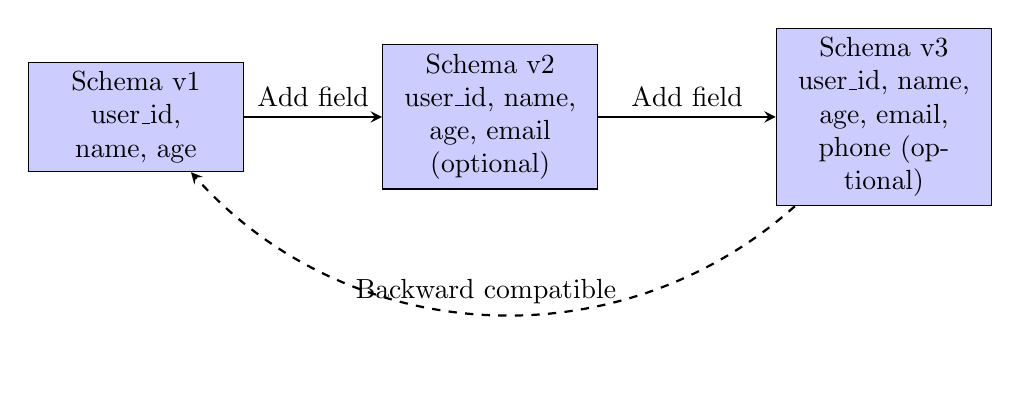
\begin{tikzpicture}[node distance=2cm]
    \tikzstyle{version} = [rectangle, draw, fill=blue!20, text width=2.5cm, text centered, minimum height=1cm]
    \tikzstyle{arrow} = [thick,->,>=stealth]

    \node [version] (v1) {Schema v1\\user\_id, name, age};
    \node [version, right of=v1, node distance=4.5cm] (v2) {Schema v2\\user\_id, name,\\age, email (optional)};
    \node [version, right of=v2, node distance=5cm] (v3) {Schema v3\\user\_id, name,\\age, email,\\phone (optional)};

    \draw [arrow] (v1) -- (v2) node[midway, above] {Add field};
    \draw [arrow] (v2) -- (v3) node[midway, above] {Add field};

    \draw [arrow, dashed, bend left=45] (v3) to node[above] {Backward compatible} (v1);
\end{tikzpicture}
\caption{Schema evolution with backward compatibility}
\label{fig:schema_evolution}
\end{figure}

\subsection{Apache Avro for Schema Management}

Avro provides schema evolution with strong compatibility guarantees:

\begin{lstlisting}[style=python, caption=Schema evolution with Apache Avro]
from avro.datafile import DataFileWriter, DataFileReader
from avro.io import DatumWriter, DatumReader
import avro.schema
import json

# Original schema v1
schema_v1_json = '''
{
  "namespace": "ml.features",
  "type": "record",
  "name": "UserFeatures",
  "fields": [
    {"name": "user_id", "type": "string"},
    {"name": "total_events", "type": "int"},
    {"name": "avg_duration", "type": "double"}
  ]
}
'''

# Evolved schema v2 (backward compatible)
schema_v2_json = '''
{
  "namespace": "ml.features",
  "type": "record",
  "name": "UserFeatures",
  "fields": [
    {"name": "user_id", "type": "string"},
    {"name": "total_events", "type": "int"},
    {"name": "avg_duration", "type": "double"},
    {"name": "user_segment", "type": ["null", "string"], "default": null},
    {"name": "premium_user", "type": "boolean", "default": false}
  ]
}
'''

class AvroSchemaManager:
    """Manage schema evolution for ML features"""

    def __init__(self, schema_registry_url: str = None):
        self.schema_registry_url = schema_registry_url
        self.schemas = {}

    def register_schema(self, name: str, schema_json: str, version: int):
        """Register a schema version"""
        schema = avro.schema.parse(schema_json)
        self.schemas[(name, version)] = schema
        return schema

    def write_features(self, filename: str, features: list, schema_version: int):
        """Write features with specific schema version"""
        schema = self.schemas[("UserFeatures", schema_version)]

        with open(filename, 'wb') as f:
            writer = DataFileWriter(f, DatumWriter(), schema)
            for feature in features:
                writer.append(feature)
            writer.close()

    def read_features(self, filename: str, reader_schema_version: int = None):
        """Read features, optionally with schema evolution"""
        features = []

        with open(filename, 'rb') as f:
            reader = DataFileReader(f, DatumReader())

            # Get writer's schema (embedded in file)
            writer_schema = reader.datum_reader.writer_schema

            # Optionally provide reader schema for evolution
            if reader_schema_version:
                reader_schema = self.schemas[("UserFeatures", reader_schema_version)]
                reader.datum_reader.reader_schema = reader_schema

            for feature in reader:
                features.append(feature)

            reader.close()

        return features

    def validate_compatibility(self, old_schema_json: str,
                              new_schema_json: str) -> dict:
        """Check schema compatibility"""
        old_schema = avro.schema.parse(old_schema_json)
        new_schema = avro.schema.parse(new_schema_json)

        compatibility = {
            'backward_compatible': self._check_backward_compatible(
                old_schema, new_schema
            ),
            'forward_compatible': self._check_forward_compatible(
                old_schema, new_schema
            )
        }

        return compatibility

    def _check_backward_compatible(self, old_schema, new_schema) -> bool:
        """Check if new schema can read data written with old schema"""
        # New schema must have defaults for any new fields
        old_fields = {f.name for f in old_schema.fields}
        new_fields_dict = {f.name: f for f in new_schema.fields}

        for field_name in new_fields_dict:
            if field_name not in old_fields:
                # New field must have default
                if not new_fields_dict[field_name].has_default:
                    return False

        return True

    def _check_forward_compatible(self, old_schema, new_schema) -> bool:
        """Check if old schema can read data written with new schema"""
        # Old schema must be able to ignore new fields
        new_fields = {f.name for f in new_schema.fields}
        old_fields_dict = {f.name: f for f in old_schema.fields}

        for field_name in old_fields_dict:
            if field_name not in new_fields:
                # Field was removed - not forward compatible
                return False

        return True

# Usage example
if __name__ == '__main__':
    manager = AvroSchemaManager()

    # Register schemas
    manager.register_schema("UserFeatures", schema_v1_json, version=1)
    manager.register_schema("UserFeatures", schema_v2_json, version=2)

    # Write data with v1 schema
    features_v1 = [
        {"user_id": "user_1", "total_events": 100, "avg_duration": 45.2},
        {"user_id": "user_2", "total_events": 200, "avg_duration": 60.1}
    ]
    manager.write_features("features_v1.avro", features_v1, schema_version=1)

    # Read v1 data with v2 schema (backward compatibility)
    features = manager.read_features("features_v1.avro", reader_schema_version=2)
    print("Features with evolved schema:", features)
    # New fields have default values: user_segment=null, premium_user=false

    # Validate compatibility
    compat = manager.validate_compatibility(schema_v1_json, schema_v2_json)
    print(f"Backward compatible: {compat['backward_compatible']}")
    print(f"Forward compatible: {compat['forward_compatible']}")
\end{lstlisting}

\subsection{Handling Breaking Schema Changes}

When breaking changes are unavoidable:

\begin{lstlisting}[style=python, caption=Managing breaking schema changes]
from typing import Any, Dict
import pandas as pd

class SchemaAdapter:
    """Adapt between schema versions for breaking changes"""

    def __init__(self):
        self.adapters = {
            (1, 2): self._adapt_v1_to_v2,
            (2, 3): self._adapt_v2_to_v3,
        }

    def adapt(self, data: pd.DataFrame,
             from_version: int,
             to_version: int) -> pd.DataFrame:
        """Adapt data from one schema version to another"""

        if from_version == to_version:
            return data

        # Apply series of adaptations
        current_version = from_version
        current_data = data.copy()

        while current_version < to_version:
            adapter_key = (current_version, current_version + 1)
            if adapter_key not in self.adapters:
                raise ValueError(
                    f"No adapter from v{current_version} to "
                    f"v{current_version + 1}"
                )

            current_data = self.adapters[adapter_key](current_data)
            current_version += 1

        return current_data

    def _adapt_v1_to_v2(self, df: pd.DataFrame) -> pd.DataFrame:
        """Adapt schema from v1 to v2"""
        # v1: user_age (int) -> v2: user_age_group (str)
        df['user_age_group'] = pd.cut(
            df['user_age'],
            bins=[0, 18, 35, 50, 100],
            labels=['<18', '18-35', '35-50', '50+']
        )
        df = df.drop(columns=['user_age'])

        # Add new required field with computed default
        df['signup_year'] = pd.to_datetime(df['signup_date']).dt.year

        return df

    def _adapt_v2_to_v3(self, df: pd.DataFrame) -> pd.DataFrame:
        """Adapt schema from v2 to v3"""
        # v2: country (str) -> v3: country_code (str, ISO 3166-1)
        country_mapping = {
            'USA': 'US',
            'United States': 'US',
            'UK': 'GB',
            'United Kingdom': 'GB',
            # ... more mappings
        }
        df['country_code'] = df['country'].map(country_mapping)
        df = df.drop(columns=['country'])

        return df
\end{lstlisting}

\section{Building a Complete Data Pipeline}

Let's integrate all concepts into a production-ready data pipeline:

\begin{lstlisting}[style=python, caption=Complete production data pipeline]
from dataclasses import dataclass
from typing import List, Dict, Any
import pandas as pd
import apache_beam as beam
from apache_beam.options.pipeline_options import PipelineOptions
import great_expectations as ge
from feast import FeatureStore
import logging
from datetime import datetime

logger = logging.getLogger(__name__)

@dataclass
class PipelineConfig:
    """Configuration for data pipeline"""
    input_source: str
    output_sink: str
    feature_store_repo: str
    validation_suite: str
    schema_version: int
    enable_drift_detection: bool = True

class DataPipeline:
    """Complete production data pipeline for ML"""

    def __init__(self, config: PipelineConfig):
        self.config = config
        self.feature_store = FeatureStore(
            repo_path=config.feature_store_repo
        )
        self.validator = DataValidator('./great_expectations')

    def run(self):
        """Execute end-to-end pipeline"""
        logger.info("Starting data pipeline...")

        # 1. Extract
        raw_data = self.extract_data()
        logger.info(f"Extracted {len(raw_data)} records")

        # 2. Validate raw data
        self.validate_data(raw_data, stage='raw')

        # 3. Transform
        transformed_data = self.transform_data(raw_data)
        logger.info(f"Transformed {len(transformed_data)} records")

        # 4. Validate transformed data
        self.validate_data(transformed_data, stage='transformed')

        # 5. Engineer features
        features = self.engineer_features(transformed_data)
        logger.info(f"Engineered {len(features.columns)} features")

        # 6. Validate features
        self.validate_data(features, stage='features')

        # 7. Detect drift (if enabled)
        if self.config.enable_drift_detection:
            self.detect_drift(features)

        # 8. Write to feature store
        self.write_to_feature_store(features)

        # 9. Write to data lake
        self.write_to_lake(features)

        logger.info("Pipeline completed successfully")

        return features

    def extract_data(self) -> pd.DataFrame:
        """Extract data from source"""
        # Implementation depends on source (DB, API, files, etc.)
        df = pd.read_parquet(self.config.input_source)
        return df

    def validate_data(self, df: pd.DataFrame, stage: str):
        """Validate data at pipeline stage"""
        suite_name = f"{self.config.validation_suite}_{stage}"

        try:
            results = self.validator.validate_batch(
                suite_name=suite_name,
                df=df,
                fail_on_error=True
            )
            logger.info(f"Validation passed at stage: {stage}")
        except ValueError as e:
            logger.error(f"Validation failed at stage {stage}: {e}")
            raise

    def transform_data(self, df: pd.DataFrame) -> pd.DataFrame:
        """Clean and transform raw data"""
        df = df.copy()

        # Remove duplicates
        df = df.drop_duplicates(subset=['user_id', 'timestamp'])

        # Handle missing values
        df['page_url'] = df['page_url'].fillna('')
        df['duration_ms'] = df['duration_ms'].fillna(0)

        # Type conversions
        df['timestamp'] = pd.to_datetime(df['timestamp'])
        df['user_id'] = df['user_id'].astype(str)

        # Filter invalid records
        df = df[df['duration_ms'] >= 0]
        df = df[df['timestamp'] <= datetime.now()]

        return df

    def engineer_features(self, df: pd.DataFrame) -> pd.DataFrame:
        """Engineer ML features"""
        df = df.copy()
        df = df.sort_values(['user_id', 'timestamp'])

        # Aggregation features
        user_features = df.groupby('user_id').agg({
            'event_type': 'count',
            'duration_ms': ['mean', 'std', 'max'],
            'page_url': 'nunique',
            'timestamp': ['min', 'max']
        }).reset_index()

        user_features.columns = [
            'user_id', 'total_events', 'avg_duration', 'std_duration',
            'max_duration', 'unique_pages', 'first_event', 'last_event'
        ]

        # Temporal features
        user_features['days_active'] = (
            user_features['last_event'] - user_features['first_event']
        ).dt.days + 1

        user_features['events_per_day'] = (
            user_features['total_events'] / user_features['days_active']
        )

        # Behavioral features
        user_features['avg_session_duration'] = (
            user_features['avg_duration'] / 1000  # Convert to seconds
        )

        user_features['engagement_score'] = (
            user_features['events_per_day'] *
            user_features['unique_pages']
        )

        # Add timestamp for feature store
        user_features['feature_timestamp'] = datetime.now()

        return user_features

    def detect_drift(self, df: pd.DataFrame):
        """Detect data drift vs baseline"""
        # Load baseline data
        baseline_df = pd.read_parquet('s3://bucket/baseline_features.parquet')

        # Compute drift metrics
        drift_metrics = self.validator.monitor_data_drift(
            suite_name=self.config.validation_suite,
            baseline_df=baseline_df,
            current_df=df
        )

        # Log drift warnings
        drifted_features = [
            feat for feat, metrics in drift_metrics.items()
            if metrics['drift_detected']
        ]

        if drifted_features:
            logger.warning(
                f"Data drift detected in features: {drifted_features}"
            )
        else:
            logger.info("No significant data drift detected")

    def write_to_feature_store(self, df: pd.DataFrame):
        """Write features to online feature store"""
        self.feature_store.push(
            push_source_name="user_features_push",
            df=df,
            to="online"
        )
        logger.info("Features written to feature store")

    def write_to_lake(self, df: pd.DataFrame):
        """Write features to data lake for training"""
        output_path = f"{self.config.output_sink}/features_{datetime.now().strftime('%Y%m%d')}.parquet"
        df.to_parquet(output_path, index=False)
        logger.info(f"Features written to data lake: {output_path}")

# Pipeline orchestration with Airflow
from airflow import DAG
from airflow.operators.python import PythonOperator
from datetime import timedelta

default_args = {
    'owner': 'ml_team',
    'depends_on_past': False,
    'email_on_failure': True,
    'email': ['ml-alerts@company.com'],
    'retries': 3,
    'retry_delay': timedelta(minutes=5),
}

def run_data_pipeline(**context):
    """Airflow task to run data pipeline"""
    config = PipelineConfig(
        input_source='s3://bucket/raw/events/*.parquet',
        output_sink='s3://bucket/features/',
        feature_store_repo='./feature_repo',
        validation_suite='user_events',
        schema_version=2,
        enable_drift_detection=True
    )

    pipeline = DataPipeline(config)
    features = pipeline.run()

    # Push metrics to XCom
    context['task_instance'].xcom_push(
        key='feature_count',
        value=len(features)
    )

with DAG(
    'ml_data_pipeline_v2',
    default_args=default_args,
    description='Production ML data pipeline',
    schedule_interval='0 2 * * *',  # 2 AM daily
    start_date=datetime(2024, 1, 1),
    catchup=False,
    tags=['ml', 'features', 'production']
) as dag:

    pipeline_task = PythonOperator(
        task_id='run_pipeline',
        python_callable=run_data_pipeline,
        execution_timeout=timedelta(hours=2)
    )
\end{lstlisting}

\section{Chapter Summary}

This chapter covered the essential components of data pipeline architecture for ML systems:

\begin{itemize}
    \item \textbf{Ingestion Patterns}: Batch, streaming, and micro-batch processing with Apache Beam and Kafka
    \item \textbf{ETL vs ELT}: Trade-offs and hybrid approaches for ML workloads
    \item \textbf{Data Validation}: Comprehensive quality checks with Great Expectations and custom validators
    \item \textbf{Feature Stores}: Centralized feature management with Feast for training/serving consistency
    \item \textbf{Data Versioning}: Dataset and pipeline tracking with DVC
    \item \textbf{Schema Evolution}: Managing schema changes with Avro and compatibility strategies
\end{itemize}

Key takeaways:
\begin{enumerate}
    \item Data pipeline quality directly determines model quality
    \item Validation must occur at multiple stages: raw, transformed, features
    \item Feature stores eliminate training/serving skew
    \item Schema evolution must be planned proactively
    \item Data versioning enables reproducibility and debugging
\end{enumerate}

\section{Exercises}

\begin{exercise}
\textbf{Batch vs Streaming Decision}

Design a data pipeline for a fraud detection system that must:
\begin{itemize}
    \item Process credit card transactions in real-time (<100ms)
    \item Compute 30-day aggregate features daily
    \item Train models weekly on historical data
\end{itemize}

Specify which components should use batch vs streaming, and justify your choices. Draw an architecture diagram.
\end{exercise}

\begin{exercise}
\textbf{Implement Streaming Pipeline}

Implement a streaming pipeline using Apache Beam or Kafka that:
\begin{enumerate}
    \item Consumes clickstream events from Kafka
    \item Computes 5-minute windowed features per user
    \item Validates features using Great Expectations
    \item Writes to both online store (Redis) and offline store (S3/Parquet)
\end{enumerate}

Include error handling, dead letter queues, and monitoring.
\end{exercise}

\begin{exercise}
\textbf{Data Validation Suite}

Create a comprehensive Great Expectations suite for e-commerce transaction data:
\begin{itemize}
    \item Schema validation (types, required fields)
    \item Statistical validation (ranges, distributions)
    \item Referential integrity (user IDs exist, product IDs valid)
    \item Business rules (order amount > 0, valid payment methods)
    \item Temporal validation (timestamps in order, no future dates)
\end{itemize}

Implement custom expectations for at least 2 business-specific rules.
\end{exercise}

\begin{exercise}
\textbf{Feature Store Implementation}

Build a feature store using Feast that:
\begin{enumerate}
    \item Defines entity (user) and features (30+ day aggregates)
    \item Materializes features from offline to online store
    \item Provides <10ms feature retrieval for serving
    \item Ensures point-in-time correctness for training data
    \item Includes feature versioning and lineage tracking
\end{enumerate}

Compare performance between online and offline stores.
\end{exercise}

\begin{exercise}
\textbf{Schema Evolution}

Given this schema v1:
\begin{verbatim}
{user_id, timestamp, event_type, page_url, duration_ms}
\end{verbatim}

Design schema v2 that adds:
\begin{itemize}
    \item user\_segment (string, optional)
    \item referrer\_url (string, optional)
    \item device\_type (string, required, default="unknown")
\end{itemize}

\begin{enumerate}
    \item Implement using Avro with compatibility checks
    \item Write code to read v1 data with v2 schema
    \item Handle a breaking change: rename event\_type to action\_type
    \item Create an adapter for backward compatibility
\end{enumerate}
\end{exercise}

\begin{exercise}
\textbf{Data Drift Detection}

Implement a data drift monitoring system:
\begin{enumerate}
    \item Compute statistical properties (mean, std, quantiles) for baseline data
    \item Monitor incoming data batches for distribution shifts
    \item Detect drift using Kolmogorov-Smirnov test or similar
    \item Alert when drift exceeds threshold
    \item Visualize drift metrics over time
\end{enumerate}

Test with synthetic data where you inject distribution shifts.
\end{exercise}

\begin{exercise}
\textbf{End-to-End Pipeline}

Build a complete production data pipeline:
\begin{enumerate}
    \item Extract data from PostgreSQL (batch) and Kafka (streaming)
    \item Validate with multiple Great Expectations checkpoints
    \item Engineer 50+ features using window functions
    \item Write to feature store (online + offline)
    \item Version data with DVC
    \item Orchestrate with Airflow
    \item Monitor with Prometheus metrics
    \item Handle failures with retries and alerting
\end{enumerate}

Document SLAs: latency, throughput, availability, data freshness.
\end{exercise}

\begin{exercise}
\textbf{Performance Optimization}

Given a slow batch pipeline processing 10TB daily:
\begin{enumerate}
    \item Profile the pipeline to identify bottlenecks
    \item Optimize with partitioning, compression, and caching
    \item Implement incremental processing
    \item Add parallel processing where possible
    \item Compare performance before/after optimizations
\end{enumerate}

Target: 50\% reduction in processing time and cost.
\end{exercise}
